\documentclass[t,hyperref={pdftex,unicode}]{beamer}  % [t], [c], или [b] --- вертикальное выравнивание на слайдах (верх, центр, низ)

%%% Работа с русским языком
\usepackage{cmap}					% поиск в PDF
\usepackage{mathtext} 				% русские буквы в формулах
\usepackage[T2A]{fontenc}			% кодировка
\usepackage[utf8]{inputenc}			% кодировка исходного текста
\usepackage[english,russian]{babel}	% локализация и переносы


\title{Идеальный ужин в \LaTeX :-)}
\author{Andrey G.}
\date{\today}

\usetheme{Berkeley}
\usecolortheme{crane}

\begin{document}

% Титульный слайд №1
%\frame[plain]{\titlepage}
% или
\begin{frame}
\maketitle
\end{frame}

\section{Разбор полётов}

% Слайд №2
\begin{frame}
	\frametitle{\insertsection}
	Итак, какой он - правильный ужин? \pause
	\begin{itemize}
	\item Должен легко усваиваться и полностью перевариться до того, как ты ляжешь спать. \pause
	\item Обязан быть за 4 часа до сна. Ведь ночью твоя пищеварительная система должна отдыхать, а не переваривать белки-жиры-углеводы. \pause
	\item Не может быть высококалорийным, содержать большое количество жира и углеводов. \pause
	\item Не должен утомлять тебя, уставшую, долгим приготовлением.
	\end{itemize}
	
\end{frame}

\section{Вкусный и здоровый ужин}

\subsection{Салат <<Радость>> с огурцами и сыром}

% Слайд №3
\begin{frame} [allowframebreaks]
	\frametitle{\insertsection}
	\framesubtitle{\insertsubsection}
	
	\begin{block}{Описание}
	Подойдёт и для самостоятельной вечерней трапезы, и для встречи гостей
	\begin{center}
	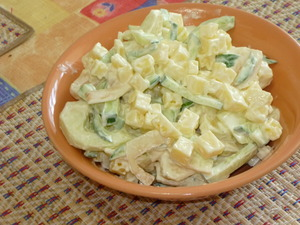
\includegraphics{6_1.jpg}
	\end{center}
	\end{block}
	
	\framebreak
		
	\begin{block}{Ингредиенты}
	\begin{enumerate}
		\item Яйцо куриное – 2 шт.
		\item Огурцы свежие – 3 шт.
		\item Лук зеленый – 2-3 пера
		\item Сыр твердый – 50 г
		\item Чеснок – 1-2 зубчика
		\item Сметана 10\% жирности – 100 г
		\item Соль, зелень – по вкусу
	\end{enumerate}
	\end{block}

\end{frame}

\subsection{Картофель по-монастырски}

% Слайд №4
\begin{frame}[allowframebreaks]
	\frametitle{\insertsection}
	\framesubtitle{\insertsubsection}
	
	\begin{block}{Описание}
	Картофель по-монастырски - это блюдо для постных дней. Маленькие хитрости - и обычное, казалось бы, блюдо заиграет новым вкусом.
	\begin{center}
		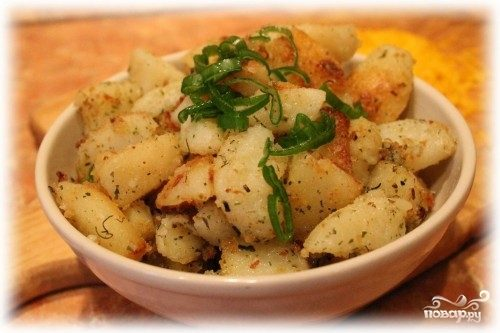
\includegraphics[scale=0.3]{6_2.jpg}
	\end{center}
	\end{block}
	
	\framebreak
		
	\begin{block}{Приготовления}
	\begin{enumerate}
		\item Картофель отварить в кожуре, охладить и почистить.
		\item Нарезать картофель или кружочками или ломтиками.
		\item Лук чистим и мелко нарезаем.
		\item Сыр твердый – 50 г
		\item Слегка обжариваем на растительном масле картофель с луком минут 5.
		\item  Посыпаем мукой, специями и солью и обжариваем до образования румяной хрустящей корочки. Не забываем в процессе жарки перемешивать картофель! 
	\end{enumerate}
	\end{block}
	
\end{frame}

\subsection{Мясные фрикадельки}

% Слайд №5
\begin{frame}[allowframebreaks]
	\frametitle{\insertsection}
	\framesubtitle{\insertsubsection}
	
	\begin{block}{Описание}
		Мясные фрикадельки - это очень легкое блюдо, которое не требует особых усилий. Все просто.
		\begin{center}
			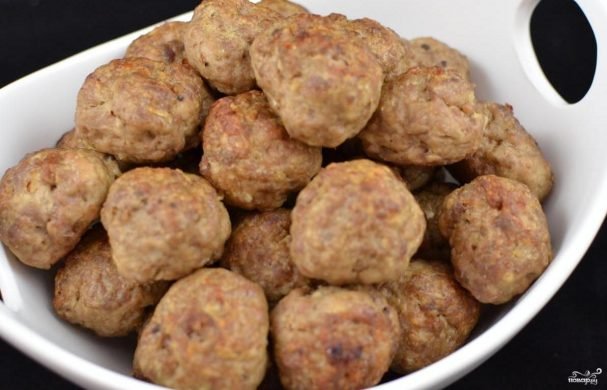
\includegraphics[scale=0.3]{6_3.jpg}
		\end{center}
	\end{block}
	
	\framebreak
	
	\begin{block}{Приготовление}
	Мясные фрикадельки - это очень легкое блюдо, которое не требует особых усилий. Все просто. Смешаем фарш с другими компонентами, даем ему настояться часик в холодильнике, затем формируем фрикадельки и готовим их. Готовить можно двумя способами - традиционным - обжарить в масле на сковородке, либо другим способом, более распространенным в Европе - запечь в духовке. Второй вариант более полезный, однако фрикадельки получаются немного суховатые и потому требуют какого-либо особенного соуса.
	\end{block}
	
	\framebreak
	
	\begin{block}{Ингридиенты}
	\begin{enumerate}
		\item Фарш — 900 Грамм (лучше всего говяжий + куриный фарш)
		\item Сметана — 1 Ст. ложка
		\item Майонез — 1 Ст. ложка
		\item Лук — 1 Штука
		\item Панировочные сухари — 1 Чашка
		\item Разрыхлитель — 1 Чайная ложка
		\item Соль, перец, молотый чеснок — - По вкусу
	\end{enumerate}
	\end{block}
	
\end{frame}

\section{Заключение}

\begin{frame}
	\frametitle{\insertsection}
	Идеальный ужин - это, прежде всего, здоровый и правильный ужин.
	Правильный ужин – это залог вашей стройности и хорошего самочувствия. Если на завтрак Вы еще можете позволить себе немного «расслабиться» и съесть что-нибудь высококалорийное и не особо полезное , то ужин – это святое. Он всегда должен быть легким, здоровым и обязательно низкокалорийным. 
	
	Подробнее о здоровом ужине можно  почитать \href{http://www.diets.ru/article/1093551/}{\beamerbutton{тут}}
\end{frame}

\end{document}